%----------------------------------------------------------------------------
\chapter{Jegyzőkönyv}
%----------------------------------------------------------------------------


%----------------------------------------------------------------------------
\section{A megadott nemlineáris függvény}
%----------------------------------------------------------------------------


Első feladatként megvalósítottuk a mérésvezető által megadott nemlineáris függvényt, amit a feladat során approximálnunk kellett. A függvény a következő volt: 

\begin{equation}\label{key}
Y = cos(\frac{X1-X2}{3}) - sin(\frac{X1+X2}{3}) + cos(\frac{X1.*X2}{8})
\end{equation}
A bemeneti változók a megadottak szerint a $ [0; 4\pi] $ intervallumon voltak, amihez a \textit{linspace} függvényt használtuk. Létrehoztuk a szükséges rácsot a \textit{meshgrid} függvénnyel, majd kirajzoltuk azt, melynek eredménye a \figref{fgv}~ábrán látható. 

\begin{figure}[!h]
	\centering
	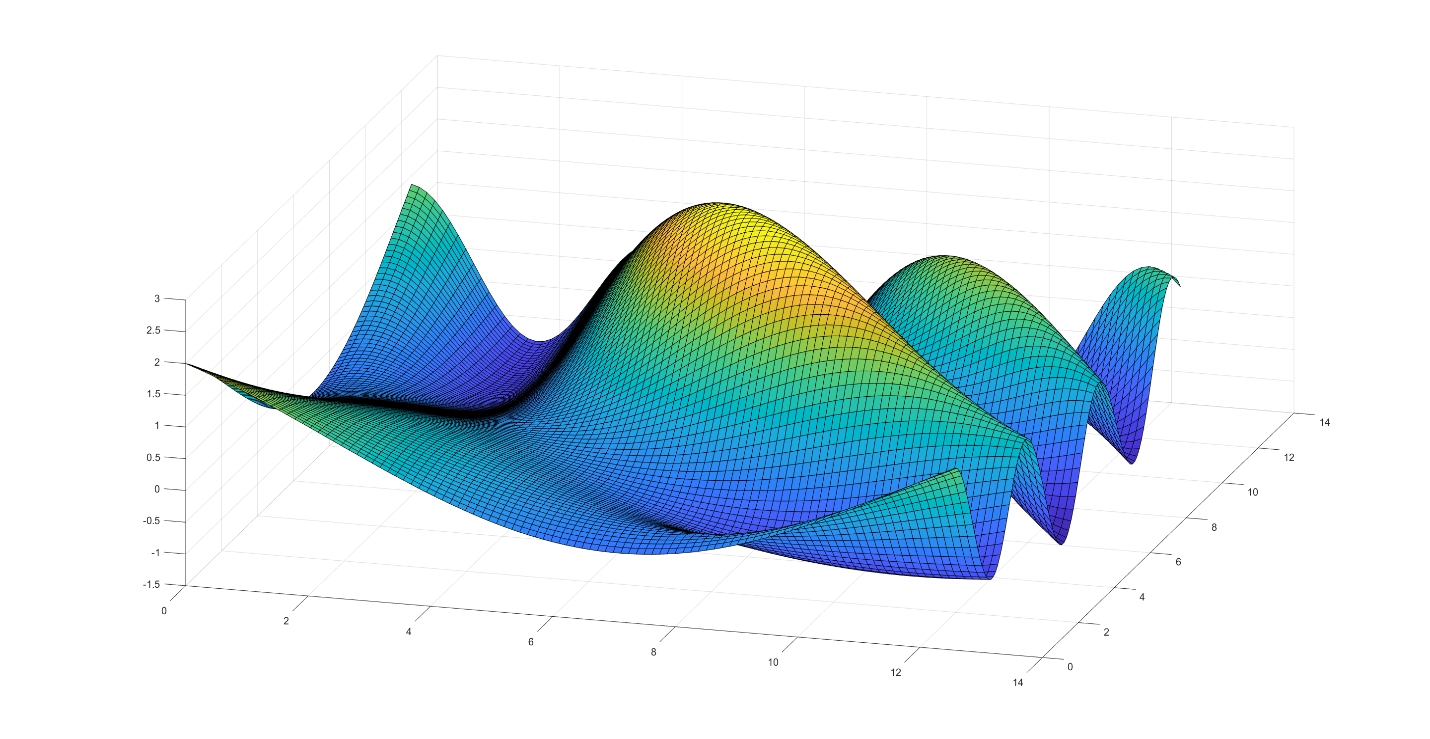
\includegraphics[width=150mm, keepaspectratio]{figures/m04/fig1.png}
	\caption{A megadott nemlineáris függvény} 
	\label{fig:fgv}
\end{figure}

Ezután a rácspontokat megkevertük, hogy a tanulásnál az algoritmusunk ne egymás melletti pontokat használjon. 
\newpage
\lstinputlisting[style=Matlab-editor]{figures/m04/matlab-1.m}\label{Matlab1}

%----------------------------------------------------------------------------
\section{Függvényapproximációs módszerek}
%----------------------------------------------------------------------------

A három lehetséges függvény közül mi a \textit{legközelebbi szomszéd alapú klaszterezést}(\textbf{fNNC}) és a \textit{fuzzy rendszer tanítását hiba-visszaterjesztéssel} (\textbf{fBP}) valósítottuk meg. 

A függvényben a bemeneti adatok és a \textit{tr} alapján meghatároztuk, hogy mik legyenek a teszt és mik a tanító adatok, majd megadtuk a tagsági függvények középpontját (első M elem a bemeneti pontokból). A szórást az az $ \frac{xMax–xMin}{M} $ képlettel számoltuk.
\lstinputlisting[style=Matlab-editor]{figures/m04/matlab-2.m}\label{Matlab2}

Ezt követően a \textit{tau} mátrixba összefoglaljuk a tagsági függvényeket, majd kiszámítjuk a kimenet paraméterfüggését, azaz az egyes deriváltakat. Frissítjük a paramétereket és kiírjuk az eredményeket, a hibát. 
\lstinputlisting[style=Matlab-editor]{figures/m04/matlab-3.m}\label{Matlab3}

\newpage
M értéknek egy viszonylag nagy értéket, 50-et választottunk, mivel a függvény bonyolult volt. Hogy ne rekedjünk meg a pontosság javulásában egy kicsi számot választottunk tanulási rátának, 0.05-öt.

Eredmény 50 ciklus után:
\begin{lstlisting}[frame=single]
50. iteracio:
Hibaosszeg: 290.6567
Legnagyobb hiba: 0.77082
Atlagos hiba: 0.032295
Negyzetes hiba: 0.0011209
\end{lstlisting}

A tesztelés eredménye:
\begin{lstlisting}[frame=single]
TESTING
Hibaosszeg: 30.3896
Legnagyobb hiba: 0.44769
Atlagos hiba: 0.030359
Negyzetes hiba: 0.00090544
\end{lstlisting}

A legközelebbi szomszéd alapú függvény implementációja:
\lstinputlisting[style=Matlab-editor]{figures/m04/matlab-4.m}\label{Matlab4}


























